% !TeX root = ../main.tex

\chapter{实验部分}\label{equations}
为了验证本文提出的加速 NeRF 的方法的有效性,本章将详尽地描述所做的相关的验证性和解释性实验,首先将本文提出的方法命名为 F-NeRF。首先将介绍实验的基本设置,包含使用的深度学习框架、开发语言、训练集和测试集,其次给出 F-NeRF 在合成新视图这样任务上的基本效果,然后详尽地描述 F-NeRF 的预训练过程,训练过程,相关参数配置,接着描述 F-NeRF 在合成数据集 Synthetic-NeRF 和真实场景数据集 LLFF-NeRF 上的实验效果以及分析。最后根据实验效果给出实验结论并进行总结。
\section{实验基本设置}\label{experiment-set}
首先先介绍下本文实验的基本设置,包含开发环境和实验所需的数据集。
\subsection{开发环境}
现如今的深度学习框架有很多,包含Caffe、Tensorflow和Pytorch等。Caffe是基于 C++ 语言开发出的深度学习框架,当然也提供 python 的接口,核心是使用 C++ 开发的,也因此更高效,适合工业界开发,但它缺少灵活性和拓展性,环境配置复杂。Tensorflow 是目前应用最广泛的深度学习框架,由谷歌公司开发与维护,具有十分成熟的社区与工具,已经广泛地被应用到企业中了。Pytorch 是相对较新的深度学习框架,由 Facebook 开发与维护的,以代码简洁上手容易,容易实现并行等优点进入到开发者的视野中,现在越来越受到学术界和工业界的青睐。由于查询表使用 Pytorch 实现更为简便,所以本文使用 Pytorch 来实现神经辐射场的所有结构。使用其他框架也可以完全复现本文的方法。本文基于 Ubuntu 18.04操作系统进行开发,开发语言为 python 3.6。使用的 GPU 是一张显存为12GB的 NVIDIA Titan X。 
\subsection{数据集} \label{Dataset}
在整个新视图合成的实验中,本文使用的都是广泛使用的公开的数据集,包含合成数据集 Synthetic-NeRF 和真实世界数据集 LLFF-NeRF。下面将大致介绍下这两种数据集。
\begin{enumerate}
    \item[1)] Synthetic-NeRF 数据集:这个合成数据集是 NeRF 生成并使用的,包含由 blender 渲染的八个物体,每一张图都是$800 \times 800$的分辨率。本文为了加速训练的过程,实验中实际使用的是下采样到$400 \times 400$分辨率的图像。对于每一个物体,有100个视角作为训练集,200个新视角作为测试集。Synthetic 数据集的优点是,它拥有绝对准的相机位姿,这能够排除受位姿影响而带来的质量的下降。如图~\ref{fig:Chairs} 是该数据集的示意图。
    \item[2)] LLFF-NeRF 数据集:这个真实数据集包含八个前向场景的图像,其中五个来自于 LLFF\cite{mildenhall2019local},三个来自于 NeRF。每个场景包含20到62张图,其中$1/8$用作测试。所有的图像都有着$1008 \times 756$的高分辨率。本文为了加速训练的过程,实验中实际使用的是下采样到$504 \times 378$分辨率的图像。如图~\ref{fig:T-Rex} 是该数据集的示意图。
\end{enumerate}

\begin{figure}[thbp]
    \centering
    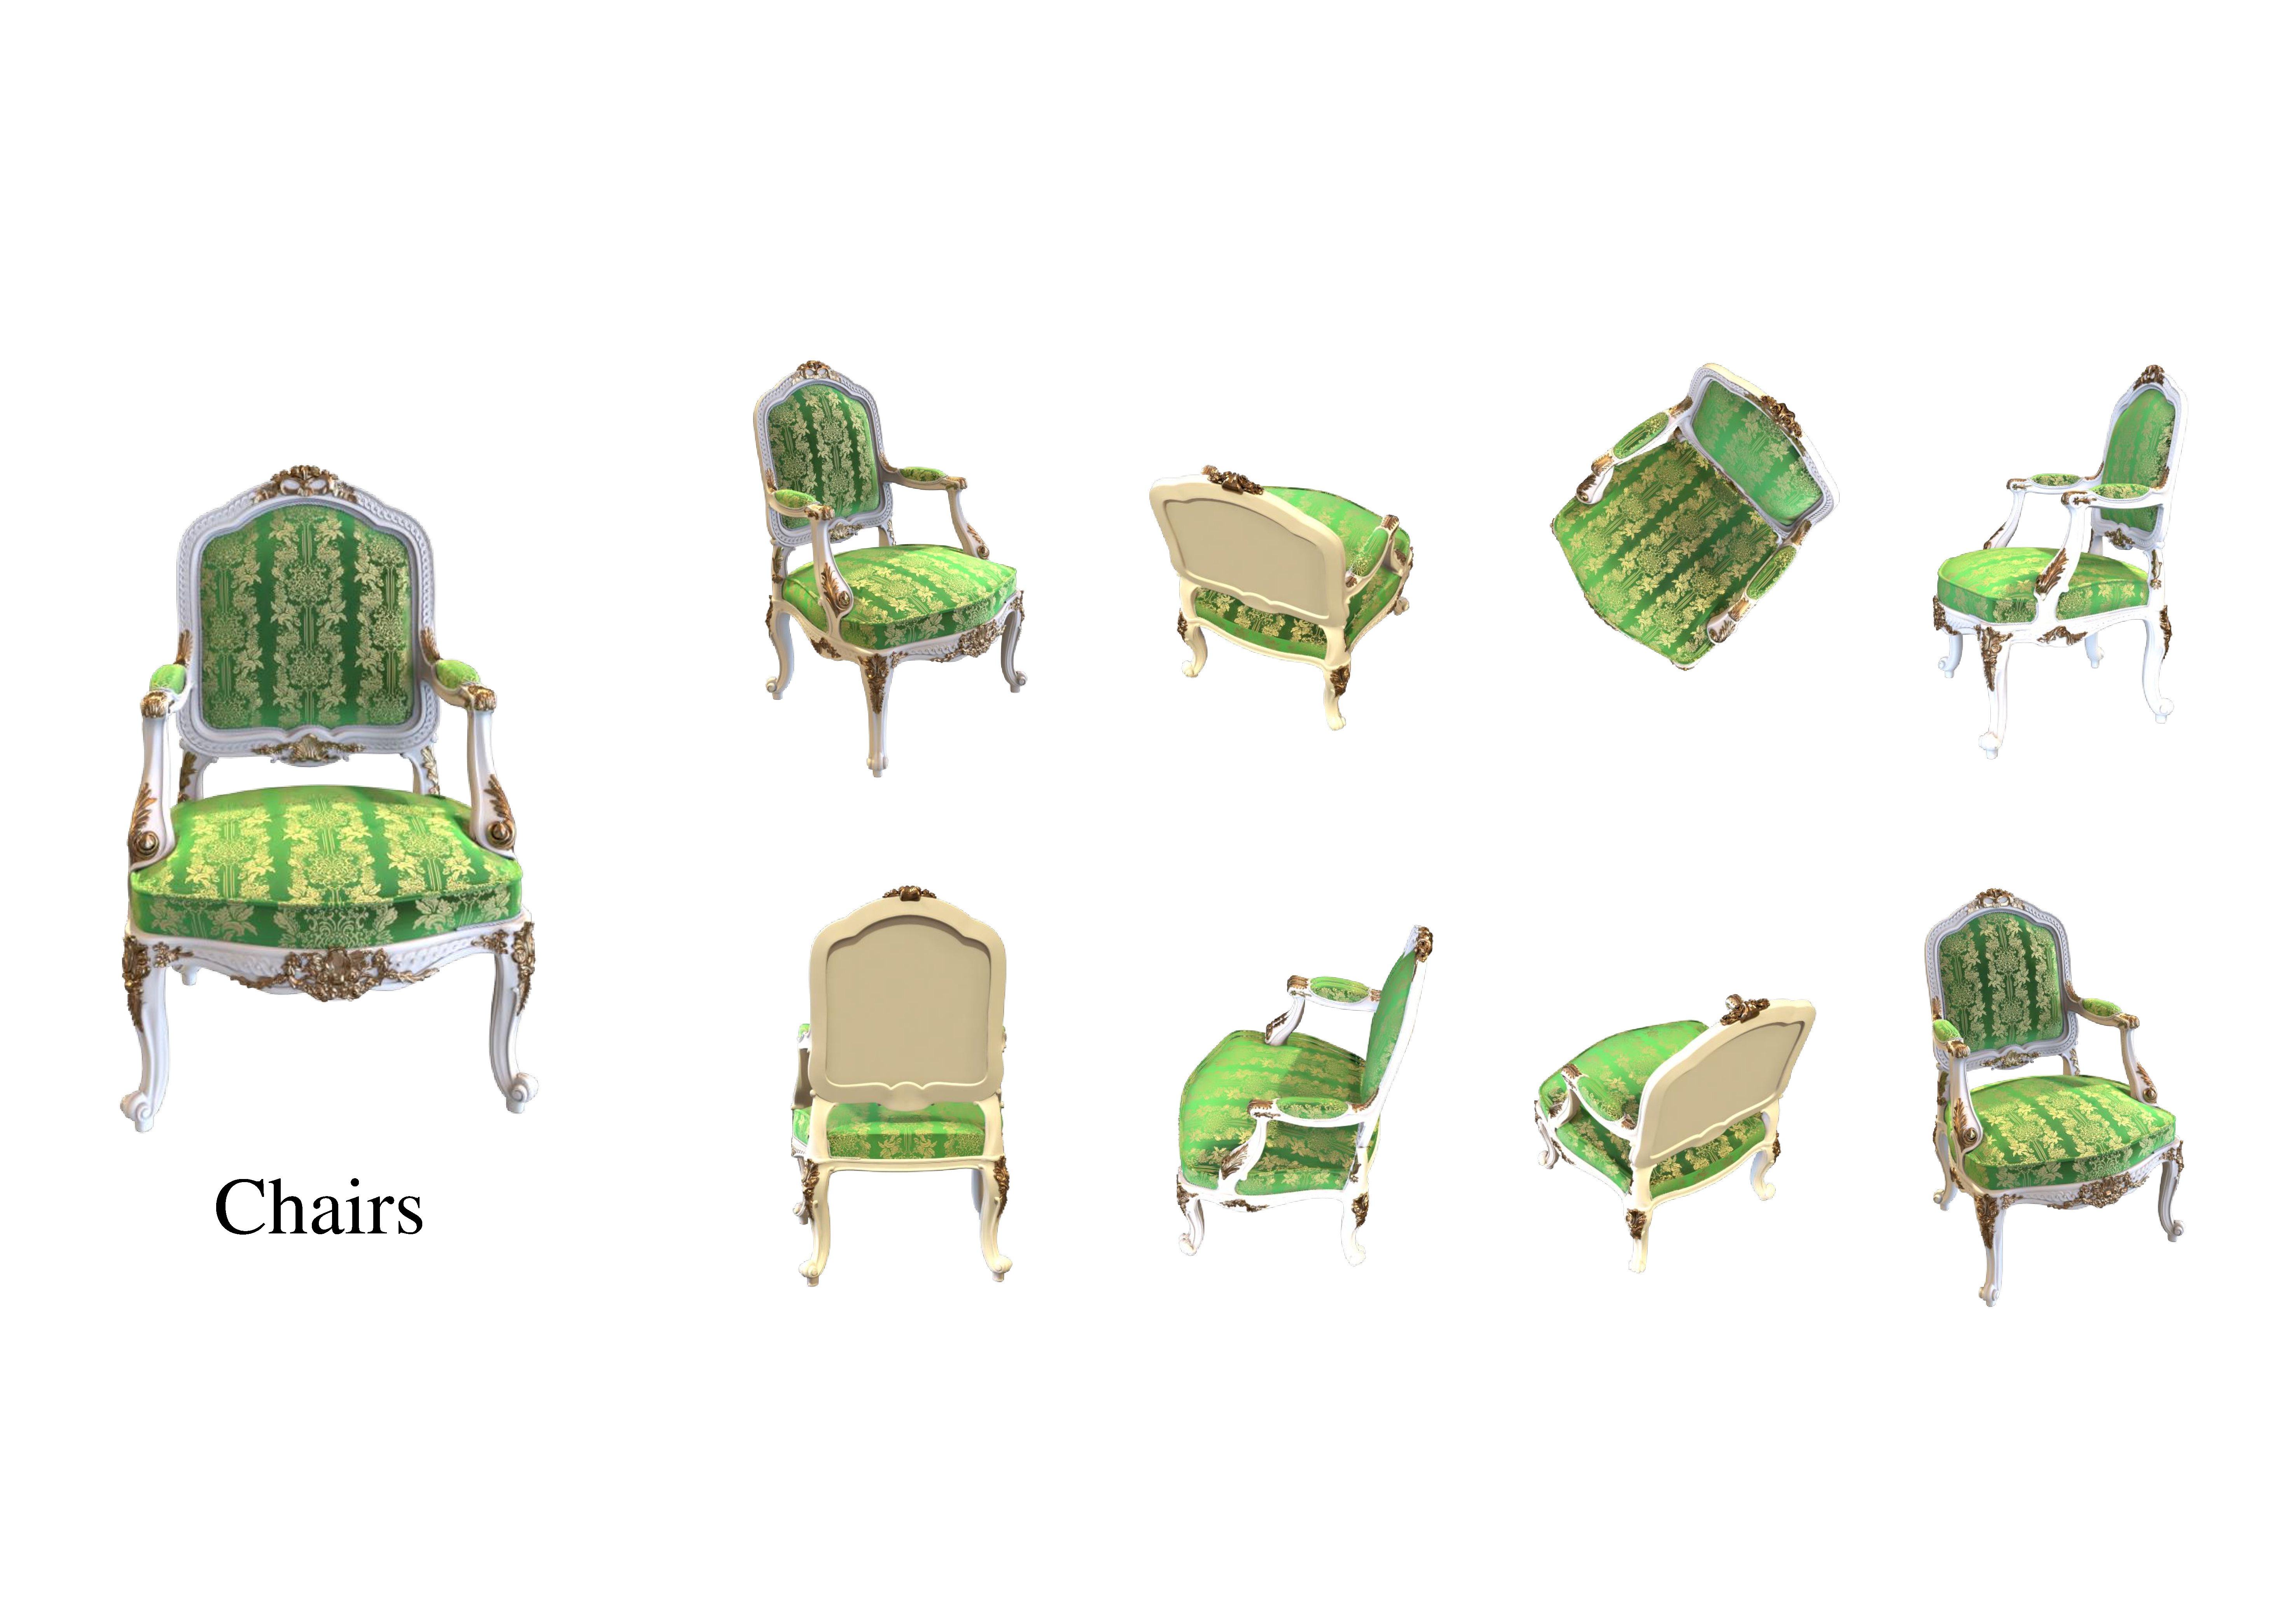
\includegraphics[width=0.95\textwidth]{figures/Chairs.pdf}
    \caption{Synthetic-NeRF 数据集示意图,第一行是部分训练集,第二行是部分测试集}
    \label{fig:Chairs}
\end{figure}

\begin{figure}[thbp]
    \centering
    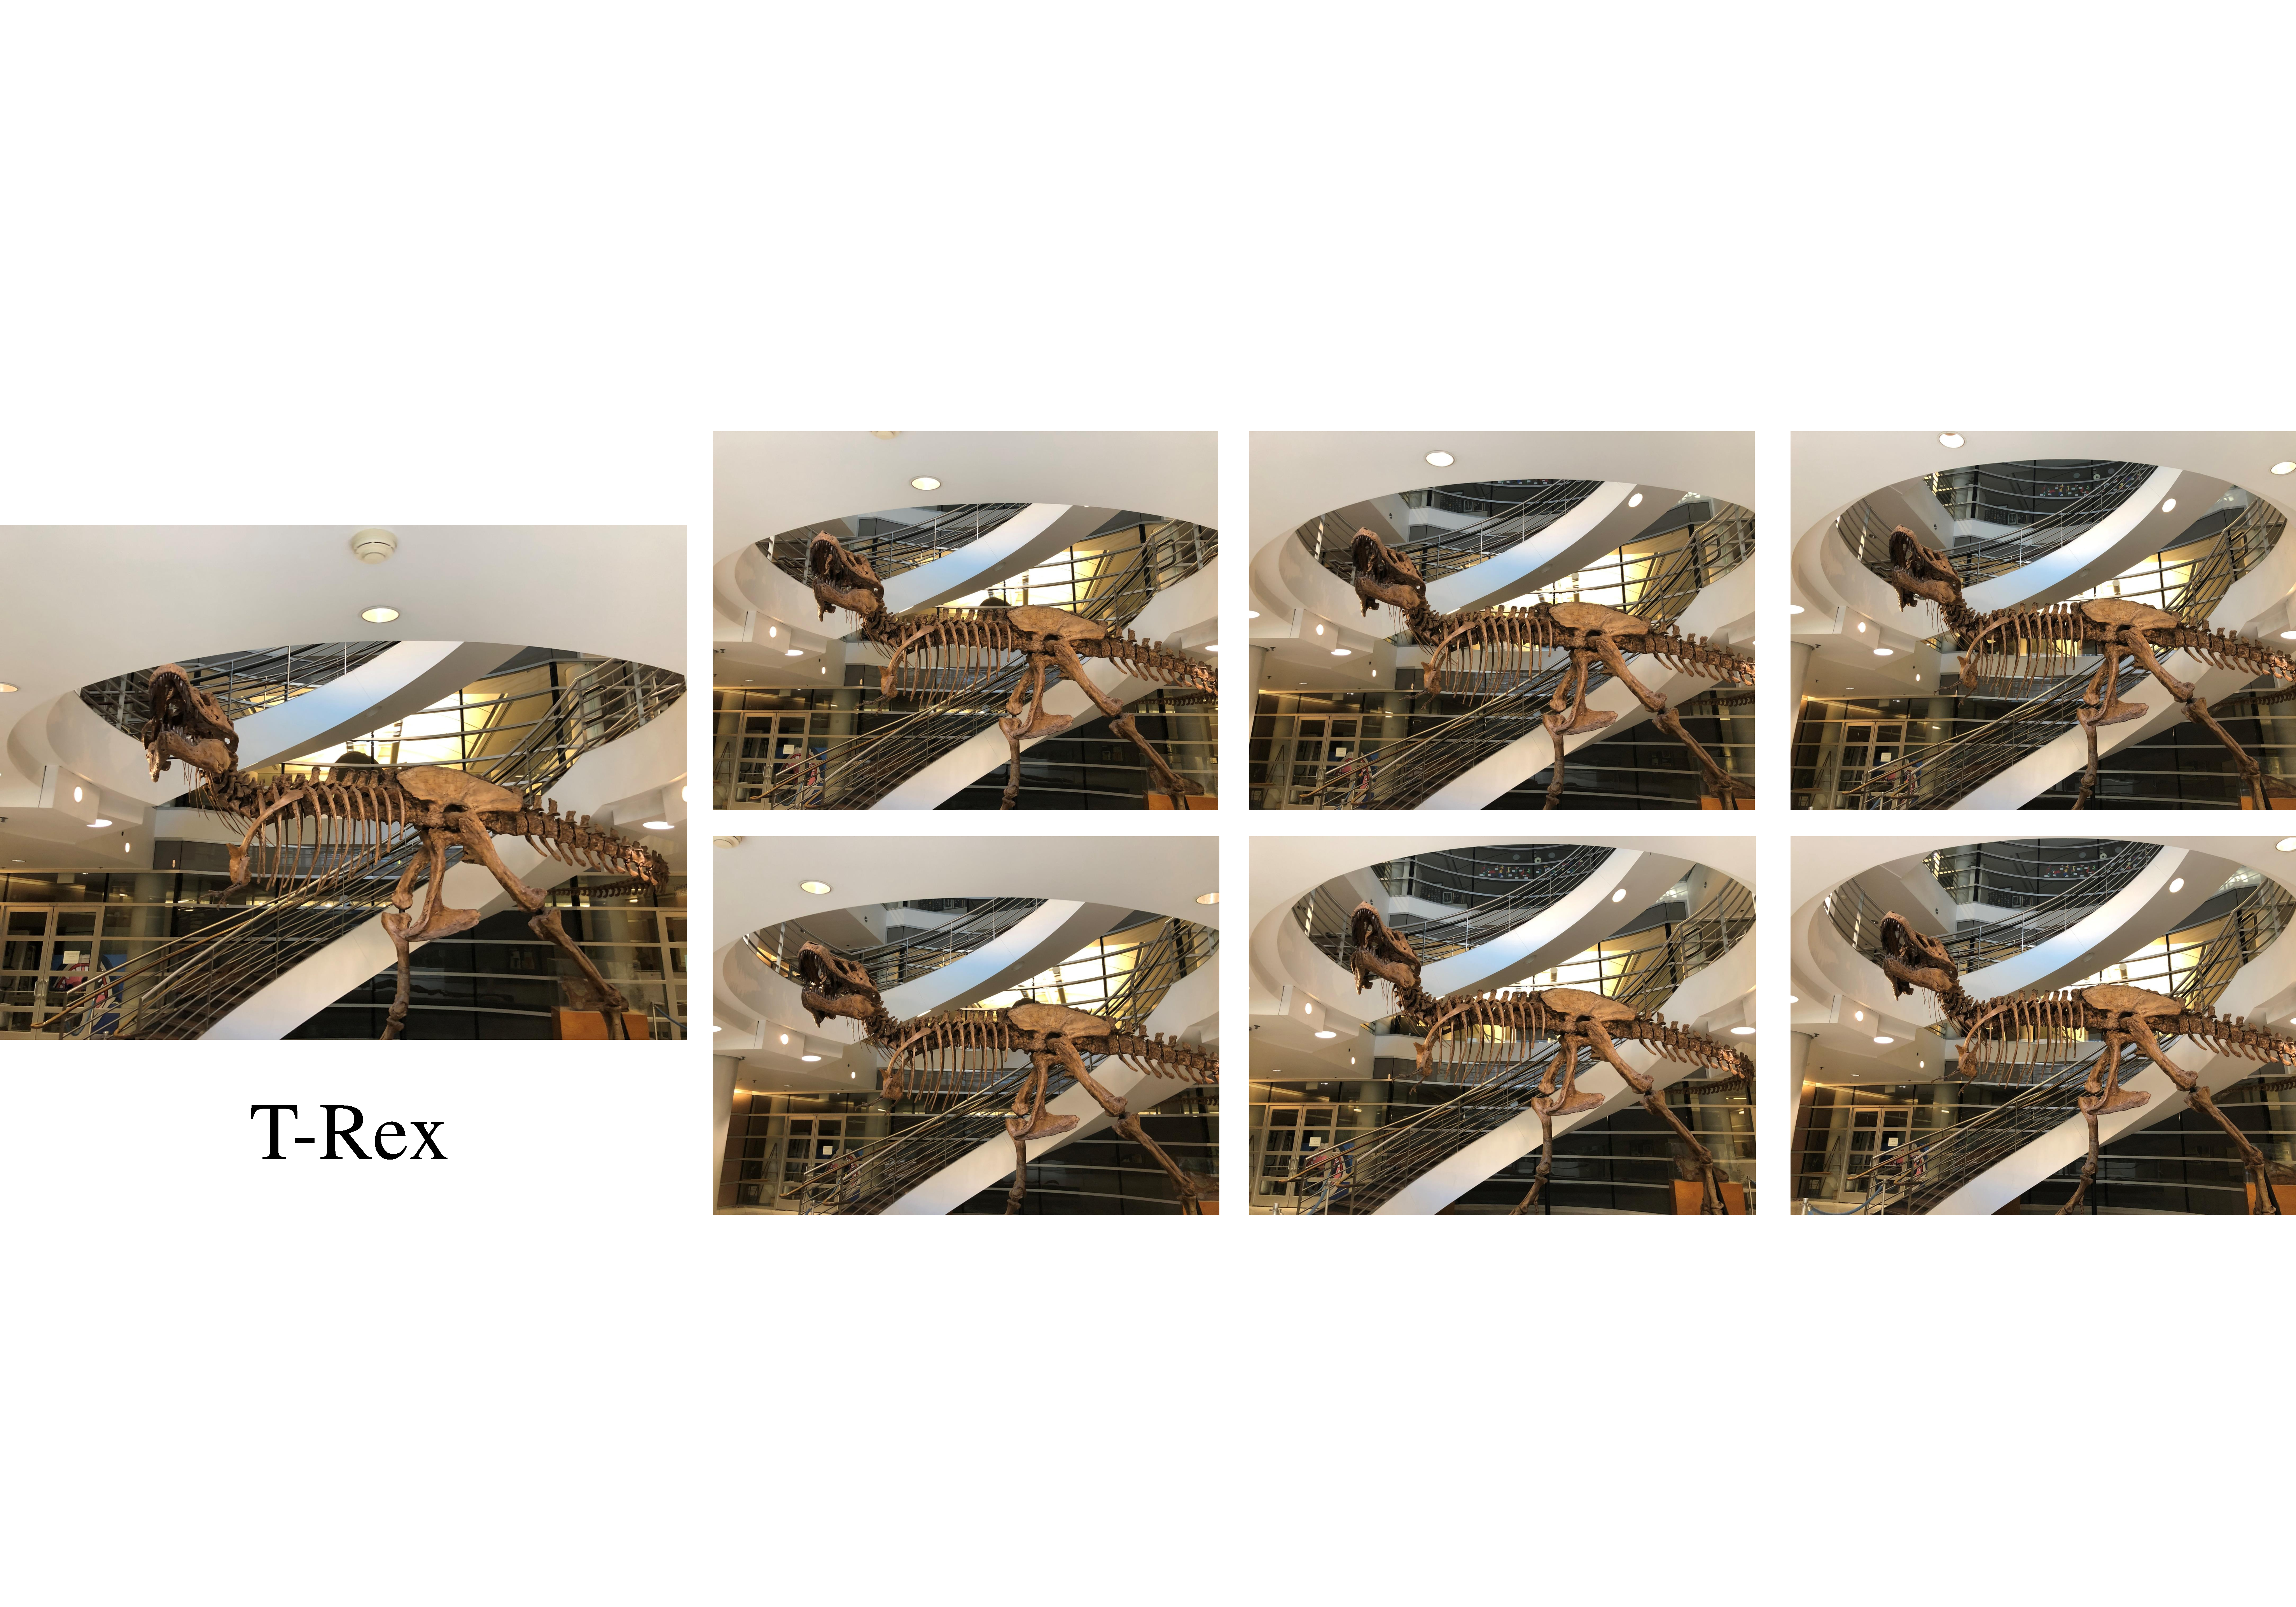
\includegraphics[width=0.95\textwidth]{figures/T-Rex.pdf}
    \caption{LLFF-NeRF 数据集示意图,第一行是部分训练集,第二行是部分测试集}
    \label{fig:T-Rex}
\end{figure}
\newpage

\section{实现细节}\label{details}
本文提出的F-NeRF架构具体见~\ref{method} 节。本文的加速模块是缓存了一张查询表,查询表的位置信息反映了物体的近似几何结构,具体缓存的是第四层全连接层输出的特征。

为了得到缓存所需的查询表,首先需要基于 NeRF 网络进行预训练,具体参数为,每个 batch 使用1024条光线,相应地,每条光线上的采样点数目为$N_c = 64$(coarse 网络),$N_f = 128$ (fine 网络)。同样地,使用 Adam 优化器\cite{kingma2014adam},在学习的过程中,学习率从$5 \times 10^{-4}$指数衰减到$5 \times 10^{-5}$(其他的 Adam 超参数使用的是默认值,$\beta_{1} = 0.9$,$\beta_{2} = 0.999$,$\epsilon = 10^{-7}$)。在合成数据集上,对每个物体的训练过程在本文的设备上大概要训练100000 epoch(大约12小时)。真实数据集上,对每个场景的训练大概200000到300000 epoch 会收敛(1到2天)。

得到了预训练的 NeRF 模型后,接下来就可以训练本文的模型 F-NeRF。首先要通过 NeRF 网络缓存一张特征查询表$T$,这个过程大概需要半分钟。为了保证质量几乎不下降,由于本文提出的 F-NeRF 模型只使用了一个网络,那么再使用 coarse 网络的64个采样点就不足以从查询表中探测到物体表面,因此,为了权衡速度与质量,F-NeRF 使用了$N = 128$个采样点,这显然仍然少于$N_c + N_f = 192$。在另一个加速的部分,F-NeRF 使用缓存的$T$替换网络的前四层全连接层,这样在测试的过程中就可以直接从缓存中获取特征,这大大减少了时间开销。以上加速模块的引入显然会导致质量的下降,第一点,去掉了一个 coarse 网络,减少了采样点,第二点,使用了缓存的特征查询表的近似特征,因此,为了保证质量不下降,必须对 F-NeRF 网络进行再训练,两个数据集大约训练100000 epoch 网络可以收敛,将近4小时。

在测试时,本文的方法和 NeRF 一样都需要一组相机参数作为输入,作用于输出图像的每个像素发出的光线上。沿着每条相机光线生成的大量采样点按照 NeRF 的理论进行积分。然而 F-NeRF 能够使用缓存的特征查询表对单网络的采样点进行优化。为了提升性能,本文对将第一次的均匀采样点送入到缓存的查询表中进行查询(使用的是最近邻的插值方式),由于查询表表征的是物体的几何结构表面,因此沿着光线找到第一个击中物体表面的点(或缓存命中),以此为中心在适当范围内进行二次均匀采样,之后将新采样点送入网络,第一步加速完成。为了进一步提升效率,F-NeRF 借助了 justlookup \cite{lin2019justlookup}的思想,查询表缓存的是原 NeRF 网络前四层输出的特征,采样点可以直接通过最近邻内插法在查询表内查询相应的特征,而减少了网络的正向传播层数,这大大加快了渲染的速度。本文的未压缩前的查询表对应的分辨率大小为$200^3$,这是实验硬件设备可支持的最大分辨率。$200^3$分辨率的查询表实质上对应着 \SI{7.63}{GB} 的内存开销,但是经过本文方法进行压缩后,平均仅需要 \SI{0.97}{GB},有效地去除空白的自由空间,这极大地节省了内存,同时也使得查询表隐藏着场景的几何信息。

\section{评测指标}\label{metrics}
\subsection{图像质量指标}
为了评估合成的新视图的质量,实质都是计算合成图像与真实观测的图像之间的差异度。假定合成图像为$\symbf{Y}$,真实图像为$\symbf{X}$,图像均为$M \times N$的彩色三通道图像,假设每个像素使用八位来存储,即像素值范围为$\left[0, 255\right]$。本文使用的质量评估指标如下:
\begin{enumerate}
    \item [1)]峰值信噪比 (Peak Signal to Noise Ratio, PSNR) \\ PSNR 是一个信号处理学科上的概念,物理含义是信号可能的最大功率与噪声功率的比值,一般使用对数分贝来表示。对于图像的情形,可以有以下公式:
    \begin{align}\label{psnr}
        \symup{PSNR} &= 10\log_{10}\left(\frac{255^{2}}{\symup{MSE}^{2}}\right), \nonumber\\
        \textit{其中均方误差} \quad \symup{MSE} &= \frac{1}{3MN}\sum_{R,G,B}\sum_{i = 0}^{M - 1}\sum_{j = 0}^{N - 1}\left[\symbf{X}\left(i,j\right) - \symbf{Y}\left(i,j\right)\right]^{2},
    \end{align}
    PSNR 是相对客观的指标,他是逐像素计算的。由公式~\ref{psnr} 可以看出,PSNR 值越大,对应 MSE 越小,那么合成图像和真实图像直接的差异也就越小。所以,PSNR 这一指标在一定程度上可以反映图像质量的好坏,但是它是比较客观的,不太涉及人眼观感,因此 PSNR 值越大,在人眼看来可能不一定好。所以在对比图像质量的时候,仅仅使用 PSNR 是不够的。\\
    \item [2)]结构相似性度量 (Structural Similarity Index Measure, SSIM\cite{wang2004image}) \\
    结构相似性的基本理念是认为图像是高度结构化的,图像之间的相邻像素有着很强的关联性。人类的视觉系统已经习惯了这种很强的结构化信息,因此在衡量图像质量的时候,推荐使用 SSIM 这一度量指标。具体地:
    \begin{equation}
        \symup{SSIM}\left(X, Y \right) = \left[l\left(\symbf{X}, \symbf{Y}\right) \right]^{\alpha} \cdot \left[c\left(\symbf{X}, \symbf{Y}\right) \right]^{\beta} \cdot \left[s\left(\symbf{X}, \symbf{Y}\right) \right]^{\gamma},
    \end{equation}
    其中$l\left(\symbf{X}, \symbf{Y}\right)$,$c\left(\symbf{X}, \symbf{Y}\right)$ 和$s\left(\symbf{X}, \symbf{Y}\right)$定义如下:
    \begin{align}
        l\left(\symbf{X}, \symbf{Y}\right) &= \frac{2\mu_{x}\mu_{y} + C_{1}}{\mu_{x}^{2} + \mu_{y}^{2} + C_{1}}, \\
        c\left(\symbf{X}, \symbf{Y}\right) &= \frac{2\sigma_{x}\sigma_{y} + C_{2}}{\sigma_{x}^{2} + \sigma_{y}^{2} + C_{2}}, \\
        s\left(\symbf{X}, \symbf{Y}\right) &= \frac{\sigma_{xy} + C_{3}}{\sigma_{x}\sigma_{y} + C_{3}},
    \end{align}
    这里的$l\left(\symbf{X}, \symbf{Y}\right)$、$c\left(\symbf{X}, \symbf{Y}\right)$ 和$s\left(\symbf{X}, \symbf{Y}\right)$分别是亮度、对比度、结构。此外,$\mu_{x}, \mu_{y}$是$\symbf{X}$和$\symbf{Y}$的均值,$\sigma_{x}^2,\sigma_{y}^2$分别是$\symbf{X}$和$\symbf{Y}$的方差,$\sigma_{xy}$是$\symbf{X}, \symbf{Y}$的协方差。$C_{1} = \left(k_{1} \times 255\right)^{2}$,$C_{2} = \left(k_{2} \times 255\right)^{2}$,$C_3 = \frac{C_2}{2}$。其中,$k_1, k_2$一般取0.01和0.03。实验中,$\alpha$,$\beta$和$\gamma$均置为1。SSIM 的值越大,表明合成图像与真实图像结构越相似。\\
    \item [3)]感知相似度(Learned Perceptual Image Patch Similarity, LPIPS\cite{zhang2018unreasonable}) \\
    该指标是基于深度学习的度量方法,这是借助了深度学习能够提取到更细粒度的图像特征,并进行对比,该指标比 PSNR、SSIM 更能符合人类的感知情况。感知损失的计算方式为:
    \begin{equation}
        d\left(\symbf{x}, \symbf{x}_{0}\right) = \sum_{l}\frac{1}{H_{l}W_{l}}\sum_{h, w} \left\| \symbf{w}_{l}\odot \left(\hat{\symbf{y}}_{hw}^{l} - \hat{\symbf{y}}_{0hw}^{l}\right)\right\|_{2}^{2},
    \end{equation}
    这里$\symbf{x}, \symbf{x}_{0}$是输入的图像,$l$是网络的层数,$\hat{\symbf{y}}_{hw}^{l}, \hat{\symbf{y}}_{0hw}^{l}$表示第一层网络的特征图,$\symbf{w}_{l}$为权重。上述也表明了 LPIPS 实际是计算了两张图之间的特征距离,因此值越小表征两张图像越相似。\\
\end{enumerate}

结合上述三个质量指标,分别可以从客观,结构,人类感知多个维度来评价合成图像与原图的差别,其中 PSNR 和 SSIM 是值越大质量越好,而 LPIPS 是值越小合成的图像与原图差异越小,质量越高,这样的质量评价体系更完整、更准确、也更公平。

% 为了评估本文提出的F-NeRF的质量,我们使用峰值信噪比 (Peak Signal to Noise Ratio, PSNR) ,结构相似度 (Structural Similarity, SSIM\cite{wang2004image}),以及具有人类感知的 LPIPS\cite{zhang2018unreasonable} 来将输出与 ground truth 进行对比。PSNR 是逐像素计算,用于测量两个输入图像之间的差异。 SSIM 是基于结构信息退化的感知图像质量评估。 在两个指标(PSNR和SSIM)中,值越大表示性能越好。 LPIPS是基于受过训练的网络的深层功能的最新感知度量,它与人类相似性判断更加一致,而较低的值表示更好的结果。

\subsection{渲染速度指标}
速度指标这里就比较简单,没有质量那么难以评估,因为速度是客观的,不受人的主观意识判断,常规地,可以使用时间或者帧率对速度进行表征。其中,时间是值越小越好,而帧率则相反。在本文后与实验部分,统一使用时间这一度量指标来表征速度,具体使用的单位是 s/frame,即渲染一帧所需的时间。


\begin{figure}[tbhp]
    \centering
    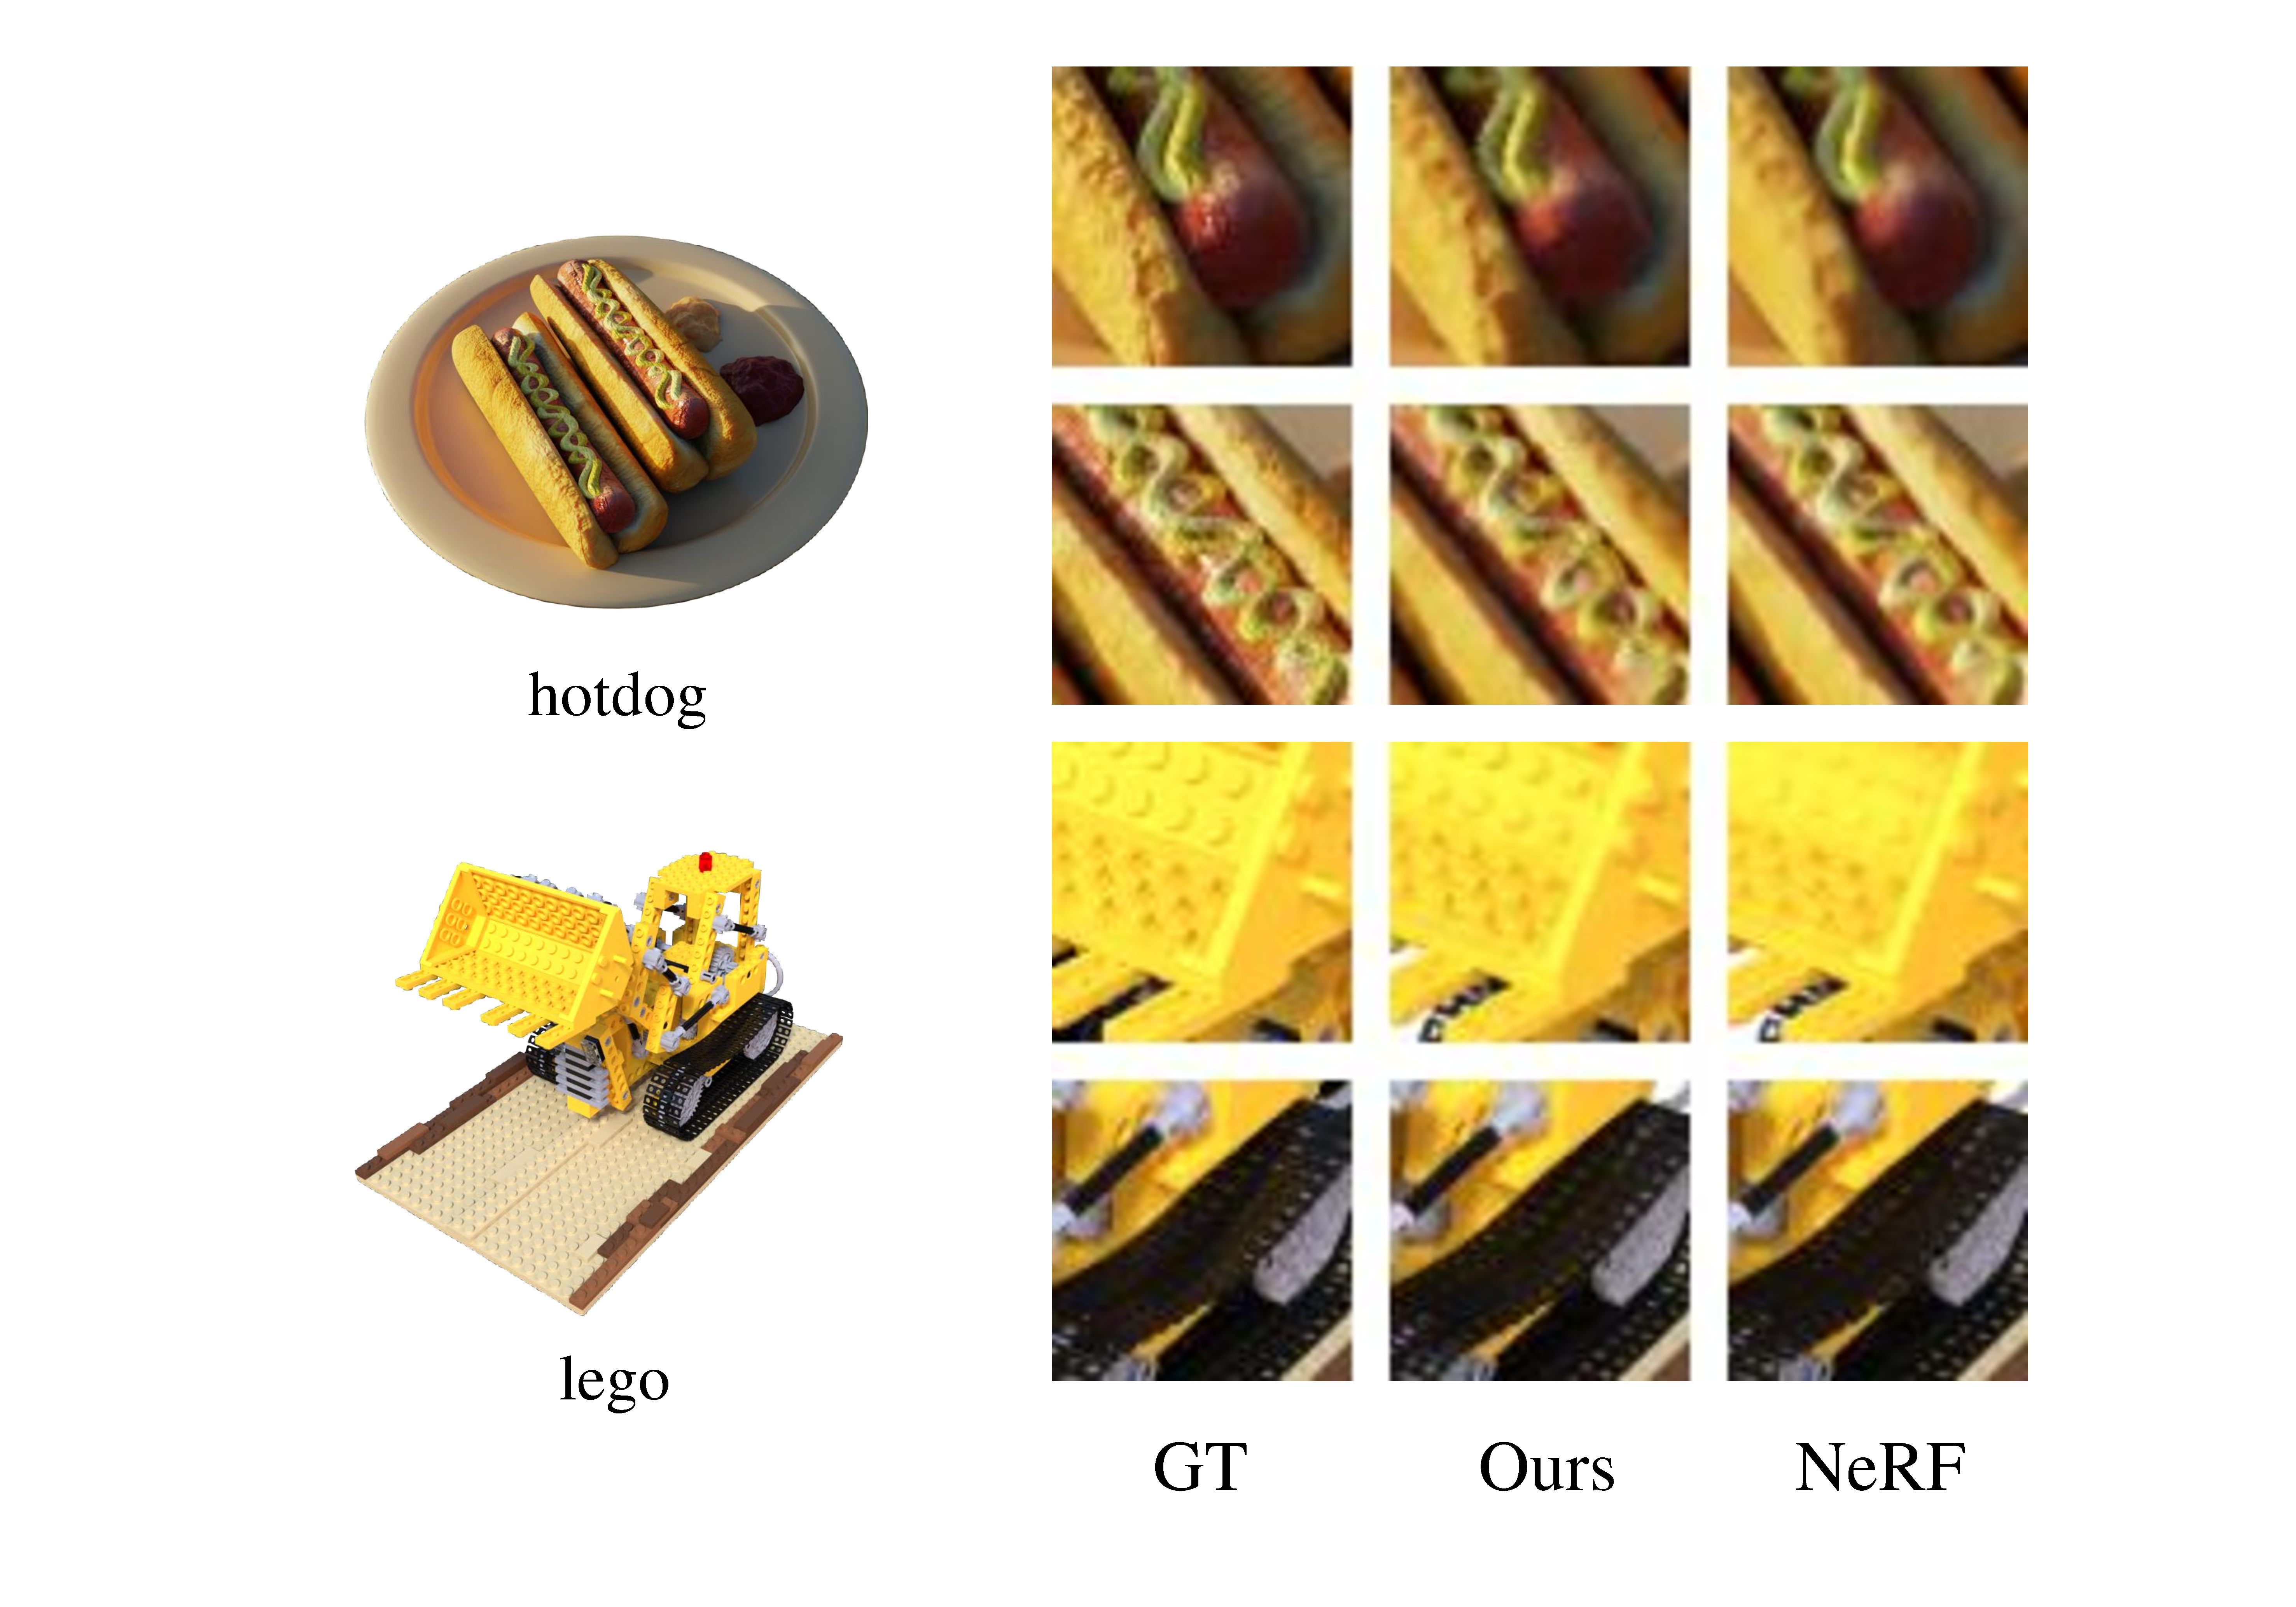
\includegraphics[width=0.95\textwidth]{figures/synthetic.pdf}
    \caption{F-NeRF 与 NeRF 在合成数据集Synthetic-NeRF上的定性比较,使用的是分辨率为$400^2$的图像。}
    \label{fig:synthetic}
\end{figure}

\begin{table}[t]
	\caption{本文提出的 F-NeRF 与 NeRF 在 PSNR,SSIM,LPIPS以及渲染一帧图像的时间上的定量对比,其中 PSNR 的单位是分贝(\si{dB}),时间的单位是秒/帧 (s/frame)}
	\label{tab:synthetic}
	\centering
	{\small\def\arraystretch{1.4}\setlength\tabcolsep{6pt}
		\begin{tabular}{cccccccccc}
			\toprule
					
			& Chair & Drums  & Ficus  & Hotdog &  Lego  & Materials & Mic & Ship & Mean\\
			\hline
			\multicolumn{10}{c}{PSNR $ \uparrow$} \\
			\hline
			NeRF   & 31.21	&\textbf{24.72}	&\textbf{28.19}	&33.03	&31.01	&28.65	&30.08	&\textbf{26.43}	&29.16\\
			\textbf{Ours} & \textbf{32.11}	&24.42	&27.84	&\textbf{35.10}	&\textbf{31.15}	&\textbf{28.79}	&\textbf{31.53}	&26.14	&\textbf{29.64}\\
			\hline
			\multicolumn{10}{c}{SSIM $ \uparrow$} \\
			\hline
			NeRF   &0.966	&\textbf{0.921}	&\textbf{0.962}	&0.958	&0.950	&0.941	&0.972	&\textbf{0.835}	&0.938\\
			\textbf{Ours} & \textbf{0.968}	&0.908	&0.955	&\textbf{0.972}	&\textbf{0.958}	&\textbf{0.951}	&\textbf{0.985}	&0.817	&\textbf{0.939}\\
			\hline
			\multicolumn{10}{c}{LPIPS $ \downarrow$}\\
			\hline
			NeRF   & 0.046	&\textbf{0.091}	&\textbf{0.044}	&0.121	&0.056	&0.063	&0.028	&\textbf{0.173}	&0.077\\
			\textbf{Ours} & \textbf{0.045}	&0.100	&0.058	&\textbf{0.044}	&\textbf{0.051}	&\textbf{0.053}	&\textbf{0.019}	&0.196	&\textbf{0.071}\\
			\hline
			\multicolumn{10}{c}{Time $ \downarrow$}\\
			\hline
			NeRF   & 15.23	&15.25	&14.89	&16.15	&15.68	&15.87	&15.01	&15.29	&15.42\\
			\textbf{Ours} & \textbf{4.71}	&\textbf{4.54}	&\textbf{4.80}	&\textbf{4.94}	&\textbf{4.84}	&\textbf{4.88}	&\textbf{4.67}	&\textbf{4.57}	&\textbf{4.74}\\
			\bottomrule
		\end{tabular}
	}
\end{table}

\newpage

\section{实验结果与分析}\label{results}
下面介绍本文的实验结果与分析部分。本文分别在公开的合成数据集 Synthetic-NeRF 和真实数据集 LLFF-NeRF 上进行了新视图合成任务的实验,上述数据集的具体细节在~\ref{Dataset} 小节。分别在这两个数据集下对实验结果进行分析。
\subsection{基于 Synthetic-NeRF 数据集的实验}
为了验证本文提出的加速方法的有效性,首先本文在公开的合成数据集 Synthetic-NeRF 的八个物体上进行了实验验证。合成数据集的场景相对简单,位姿是绝对准确的,这对于评估质量来说很有帮助。图~\ref{fig:synthetic} 给出了本文提出的 F-NeRF 与 NeRF 的定性对比结果。从结果可以看出,F-NeRF 几乎达到了和 NeRF 一样的质量,甚至在一些细节上,本文提出的 F-NeRF 还做的比较好,比如 hotdog 的沙拉酱部分,还有 lego 的铲斗部分,这一定程度上反映了本文提出的方法能够获取比较靠近表面的采样点,因为这些采样点对渲染过程的贡献更大。

表~\ref{tab:synthetic} 提供了 F-NeRF 与 NeRF 在合成数据集下的具体定量指标对比。从表格中可以看出,本文提出的方法 F-NeRF 在几乎不损失精度的情况下能够在渲染速度上为 NeRF 加速3.2倍。质量方面,F-NeRF 在 PSNR 和 SSIM 这两项指标的均值略高于 NeRF,在 LPIPS 这一指标上比 NeRF 低0.006。F-NeRF 仅在 Drums、Ficus、Ship这三个物体上的质量略低于 NeRF,这可能是因为这些物体的空洞较多,而原 NeRF 网络预测的体密度不是绝对准确的,可能会把物体内部或表面预测为物体外部而没有存在查询表中,那么该查询表就会丢失许多信息,难以把采样点的位置都约束在物体表面附近。不过,从整体上看,本文提出的 F-NeRF 几乎是达到了 NeRF 的质量水平。

以上结果表明,本文提出的新视图合成加速方法在合成数据集上能够为 NeRF 实现几乎无质量损失的显著加速。

\pagebreak
\begin{table}[htbp]
	\caption{真实世界数据集下的质量与渲染速度对比(八个场景的均值)}%
	\centering
	{\small\def\arraystretch{1.4}\setlength\tabcolsep{12pt}
			
		\begin{tabular}{lcccc}
			%\hline
			\toprule
			&PSNR (dB) \uparrow & SSIM\uparrow & LPIPS\downarrow & Speed (s/frame) \downarrow\\
			\midrule
			SRN\cite{sitzmann2019scene}         & 22.84  & 0.668  & 0.378 & -\\
			LLFF\cite{mildenhall2019local}   		 & 24.13  & 0.798  & \textbf{0.212} & -\\
			NeRF\cite{mildenhall2020nerf}   		 & 26.50  & 0.811  & 0.250 & 14.33\\
			\textbf{Ours} & \textbf{26.87}  & \textbf{0.836}  & 0.226 &\textbf{4.23}\\
			\bottomrule
		\end{tabular}
	}
		%
	\label{tab:real}
\end{table}

\subsection{基于 LLFF-NeRF 数据集的实验}
真实场景相对于合成场景更为复杂,受光照条件、相机标定等因素的影响,因此合成高质量的新视角下的图像是相对困难的。本小节将本文提出的 F-NeRF 方法应用在 LLFF-NeRF 数据集上,与目前最先进的方法 SRN\cite{sitzmann2019scene} ,LLFF\cite{mildenhall2019local},以及 NeRF\cite{mildenhall2020nerf}进行对比。真实场景的相机位姿都是通过 COLMAP \cite{schonberger2016structure} 方法计算的。

图~\ref{fig:llff} 给出了本文与 NeRF 在真实场景下的定性对比图,本文将图像中相对细节较多较复杂的部分使用红蓝框给框起来,读者可以自行放大进行对比。从图中可以看出,本文的方法在渲染的新视图的质量方面达到了几乎和 NeRF 相同的水平。具体地,对于图中的 T-Rex 场景,对应于红色框的部分,可以看出,本文的 F-NeRF 和 NeRF 都出现了细节的严重丢失,这是因为该物体过于细小,比较难采样到稳定的采样点,但事实上,F-NeRF 丢失的细节较 NeRF 还是要少一些,这是因为 F-NeRF 在采样上进行了优化,利用查询表缓存相关的几何信息,使得采样到的点是位于物体表面的对渲染贡献较高的部分。

最后表~\ref{tab:real} 给出了本文与其他方法的定量指标的对比(取八个场景的均值),可以看出本文提出的 F-NeRF 在 PSNR 上平均比 NeRF 提高\SI{0.37}{dB},在 SSIM 上能提升0.033,在 LPIPS 上能降低0.024,此外更能够给 NeRF 在渲染速度上加速3.4倍,这将使得基于神经辐射场的新视图合成系统的构建提供了可能,在下一章会具体详述本文基于 F-NeRF 所设计并实现的新视图快速合成的系统。

% 综上,以上的结果表明,本文提出的 F-NeRF 方法在真实场景中,能有效提高 NeRF 的渲染效率,同时不损失精度。 

\begin{figure}[tbhp]
    \centering
    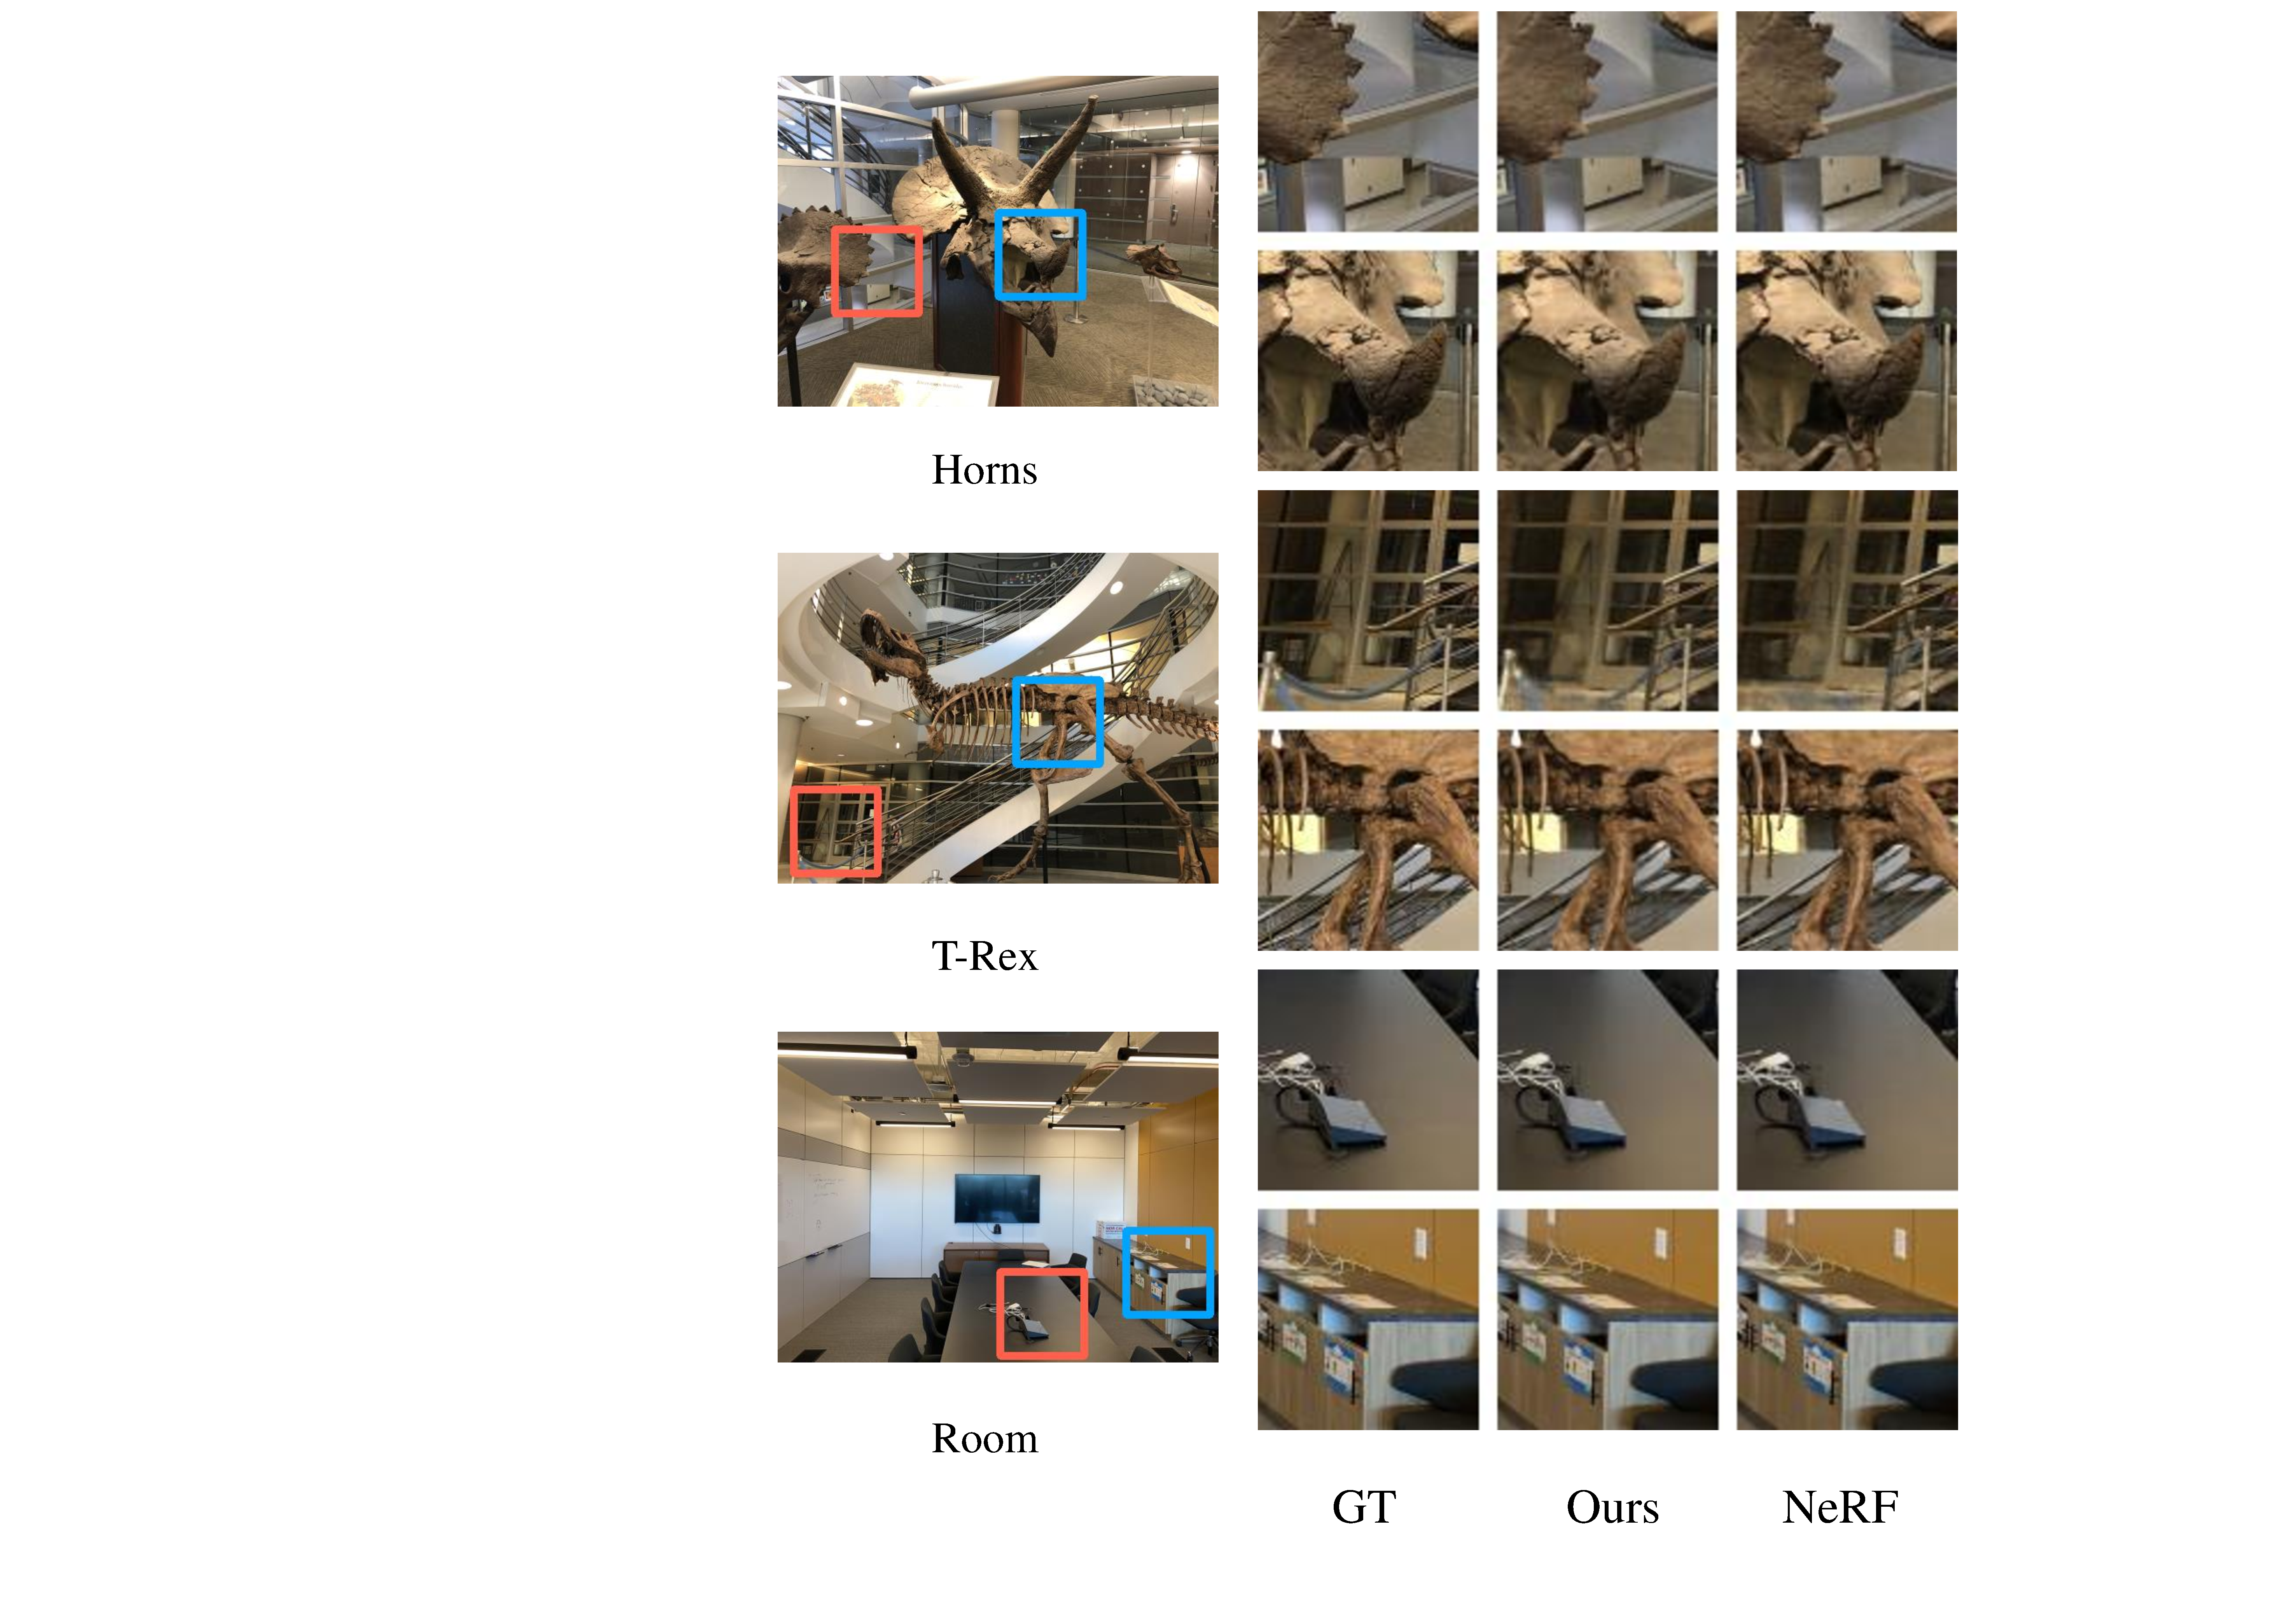
\includegraphics[width=0.95\textwidth]{figures/llff.pdf}
    \caption{F-NeRF 与 NeRF 在真实场景数据集 LLFF-NeRF 上的定性比较,使用的是分辨率为$504 \times 378$的图像。}
    \label{fig:llff}
\end{figure}
\newpage

\section{本章小结}
本章主要介绍了本文的实验部分。本章第~\ref{experiment-set} 节首先介绍了本文实验的开发环境、数据集。第~\ref{details} 节详细叙述了本文实验的一些细节,包括参数的设置,完整的训练过程,以及完整的测试过程。第~\ref{metrics} 节主要介绍了实验的具体评测指标,包含新视图合成任务中较为权威的质量评测指标,比如 PSNR、SSIM 和 LPIPS,这些指标涵盖了客观、结构相似性,以及人眼感知等多个维度去评估图像的质量,此外本节还提供了速度评估指标,主要是测试时间或渲染的帧率。最后分别基于公开的合成数据集 Synthetic-NeRF 和真实场景数据集 LLFF-NeRF, 将本文提出的方法与 NeRF 进行了性能对比,从结果上面看,本文提出的方法几乎在不损失质量的情况下对 NeRF 进行明显加速。

% \section{数学符号}

% 论文中使用的符号应符合国家标准《国际单位制及其应用》(GB 3100—1993)、《有关量、单位和符号的一般原则》(GB/T 3101—1993) 的规定。

% 要特别注意以下几点问题:

% \begin{enumerate}
% \item 数学公式结尾也不可缺少标点符号, 参见式\eqref{eq:example}, 式\eqref{eq:align}, 式\eqref{eq:equ_aligned}.
%     \item 向量、矩阵和张量要求粗斜体,应该使用 \pkg{unicode-math} 的 \cs{symbf} 命令,
%           如 \verb|\symbf{A}|、\verb|\symbf{\alpha}|。
%     \item 数学常数和特殊函数要求用正体,应使用 \cs{symup} 命令,
%     如 $\symup{\pi} = 3.14\dots$; $\symup{e} = 2.718\dots$。
%     \item 微分号和积分号使用使用正体,比如:$\int f(x) \dif x$。
%     \item 公式中的括号应写作 $\displaystyle \left(\frac{a}{b + c}\right)$, $\displaystyle \left[\frac{a}{b + c}\right]$, $\displaystyle \left\{\frac{a}{b + c}\right\}$, $\displaystyle \left<\frac{a}{b + c}\right>$, 而非 $\displaystyle (\frac{a}{b + c})$, $\displaystyle [\frac{a}{b + c}]$, $\displaystyle \{\frac{a}{b + c}\}$, $\displaystyle <\frac{a}{b + c}>$.\\
%     注意比较两种形式括号大小的区别. 在\LaTeX{}可用 \verb|\left(| $\cdot$ \verb|\right)|, \verb|\left[| $\cdot$ \verb|\right]|, \verb|\left\{| $\cdot$ \verb|\right\}|, \verb|\left<| $\cdot$ \verb|\right>| 来实现.
%     \item 关于量和单位推荐使用\href{http://mirrors.ctan.org/macros/latex/contrib/siunitx/siunitx.pdf}{\pkg{siunitx}}
% 宏包,
%         可以方便地处理希腊字母以及数字与单位之间的空白,
%         比如:
%         \SI{6.4e6}{m},
%         \SI{9}{\micro\meter},
%         \si{kg.m.s^{-1}},
%         \SIrange{10}{20}{\degreeCelsius}。
% \end{enumerate}

% \section{数学公式}

% 数学公式可以使用 \env{equation} 和 \env{equation*} 环境。
% 注意数学公式的引用应前后带括号,建议使用 \cs{eqref} 命令,比如式 \eqref{eq:example},
% \begin{equation}
%   \frac{1}{2 \symup{\pi} \symup{i}} \int_\gamma f = \sum_{k=1}^m n\left(\gamma; a_k\right) \mathscr{R}\left(f; a_k\right).
%   \label{eq:example}
% \end{equation}

% 多行公式尽可能在 ``='' 处对齐,可根据编号形式的需要使用 \env{align} 或 \env{equation}+\env{aligned} 环境, 请参考如下示例:

% \env{align}模式: 

% \begin{minipage}{.48\textwidth}
%     \begin{verbatim}
% \begin{align}
%   a & = b + c + d + e, \\
%     & = f + g.
% \end{align}
%     \end{verbatim}
% \end{minipage}
% \begin{minipage}{.48\textwidth}
%   \begin{align}\label{eq:align}
%     a & = b + c + d + e, \\
%       & = f + g.
%   \end{align}
% \end{minipage}

% \env{equation} + \env{aligned} 模式:

% \begin{minipage}{.48\textwidth}
%     \begin{verbatim}
% \begin{equation}
%     \begin{aligned}
%       a & = b + c + d + e, \\
%         & = f + g.
%     \end{aligned}
% \end{equation}
%     \end{verbatim}
% \end{minipage}
% \begin{minipage}{.48\textwidth}
%     \begin{equation}\label{eq:equ_aligned}
%         \begin{aligned}
%           a & = b + c + d + e, \\
%             & = f + g.
%         \end{aligned}
%     \end{equation}
% \end{minipage}

% \section{数学定理}

% 定理环境的格式可以使用 \pkg{amsthm} 或者 \pkg{ntheorem} 宏包配置。
% 用户在导言区载入这两者之一后,模板会自动配置 \env{thoerem}、\env{proof} 等环境。

% \begin{theorem}[Lindeberg--Lévy 中心极限定理]
%   设随机变量 $X_1, X_2, \dots, X_n$ 独立同分布, 且具有期望 $\mu$ 和有限的方差 $\sigma^2 \ne 0$,
%   记 $\bar{X}_n = \frac{1}{n} \sum_{i+1}^n X_i$,则
%   \begin{equation}
%     \lim_{n \to \infty} P \left(\frac{\sqrt{n} \left( \bar{X}_n - \mu \right)}{\sigma} \le z \right) = \Phi(z),
%   \end{equation}
%   其中 $\Phi(z)$ 是标准正态分布的分布函数。
% \end{theorem}
% \begin{proof}
%   Trivial.
% \end{proof}

% 同时模板还提供了 \env{assumption}、\env{definition}、\env{proposition}、
% \env{lemma}、\env{theorem}、\env{axiom}、\env{corollary}、\env{exercise}、
% \env{example}、\env{remar}、\env{problem}、\env{conjecture} 这些相关的环境。

\cleardoublepage
